\documentclass[uplatex,dvipdfmx]{jlreq}
\usepackage[fleqn,tbtags]{mathtools}
\usepackage{jlreq-deluxe}
\usepackage{geometry}
\usepackage{booktabs}
\usepackage{hyperref}
\usepackage[noalphabet]{pxchfon} % must be after otf package
\usepackage{stix2} %欧文＆数式フォント
\usepackage[fleqn,tbtags]{mathtools} % 数式関連 (w/ amsmath)
\usepackage{url}
\usepackage{here}
\geometry{left=20mm,right=20mm,top=25mm,bottom=25mm}

\title{作業ログ\\ \large 加速度センサーを用いた身体動作による輪唱制御システムの構築と視覚フィードバック効果}
\author{報告者: 早川　和輝}
\date{報告日: 2026年6月24日}

\begin{document}
\maketitle

\section{進捗サマリー(要約)}
\begin{itemize}
    \item 全体進捗率: [85\%]
    \item マイルストーン達成状況: [達成]
    \item 主要成果:
    \begin{itemize}
        \item 成果1: 楽器用Arduino(UNO R4 WiFi)のオンボード12$\times$8 LEDマトリクスに「ドットのカエル」を表示するコード(FrogMatrix.h)を追加．
        再生の合図で3コマのアニメーションを開始し，停止合図で消灯する．
        \item 成果2: LEDマトリクス表示を共通モジュール化し，バイオリン用とギロ用の2つのinoに同一内容で組み込んだ．
        音と同時にカエルが動き出す視覚フィードバックを実現した．
        \item 成果3: 生成した各音(ド・レ・ミ・ファ・ソ・ラ)のwavファイルについて，librosaのピッチ検出で実際の音階を解析し，目標音階との正解率を検証．
        全6音で正解率100\%を確認した．
    \end{itemize}
    \item 重大課題(影響度:無し): なし
\end{itemize}

\section{作業ログ(詳細トラッキング)}
\begin{table}[H]
    \centering
    \small
    \begin{tabular}{lp{1.5cm}p{1.5cm}llp{2.5cm}p{3cm}}
        \toprule
        作業項目 & 開始日 & 完了日 & 状態 & 進捗率 & 依存関係・ブロッカー & コメント \\
        \midrule
        LEDマトリクス表示の追加 & [6/18] & [6/22] & 完了 & 100\% & なし & UNO R4 WiFiのオンボード12$\times$8マトリクスにカエルの3コマアニメを実装．再生で開始，停止で消灯． \\
        マトリクスの共通モジュール化 & [6/22] & [6/22] & 完了 & 100\% & なし & FrogMatrix.hとしてバイオリン用・ギロ用の2つのinoに共通組み込み． \\
        音階正解率の検証 & [6/20] & [6/23] & 完了 & 100\% & なし & librosaのピッチ検出で各音を解析．6音すべてで目標音階と一致(正解率100\%)． \\
        \bottomrule
    \end{tabular}
\end{table}

\section{担当箇所の計画前のGCと現在のGC}
担当箇所である「楽器演奏実装」における，当初計画時（計画前）のガントチャート（GC）の予定と，現在の進捗・変更状況の比較である．
\begin{table}[H]
    \centering
    \small
    \begin{tabular}{lp{4cm}p{4cm}l}
        \toprule
        タスク名 & 計画前のGC（予定期間） & 現在のGC（実績・修正期間） & 進捗状態 \\
        \midrule
        テンポを変更させる処理の追加 & [6/8 $\sim$ 6/13] & [6/8 $\sim$ 6/15] & 完了 \\
        同期との連携 & [6/11 $\sim$ 6/17] & [6/11 $\sim$ 6/22] & 進行中 \\
        サーボモーターの動作確認 & [6/9 $\sim$ 6/13] & [6/9 $\sim$ 6/16] & 完了 \\
        LEDマトリクス表示の追加 & [—（新規）] & [6/18 $\sim$ 6/22] & 完了 \\
        音階正解率の検証 & [—（新規）] & [6/20 $\sim$ 6/23] & 完了 \\
        \bottomrule
    \end{tabular}
\end{table}\begin{figure}[H]
    \centering
    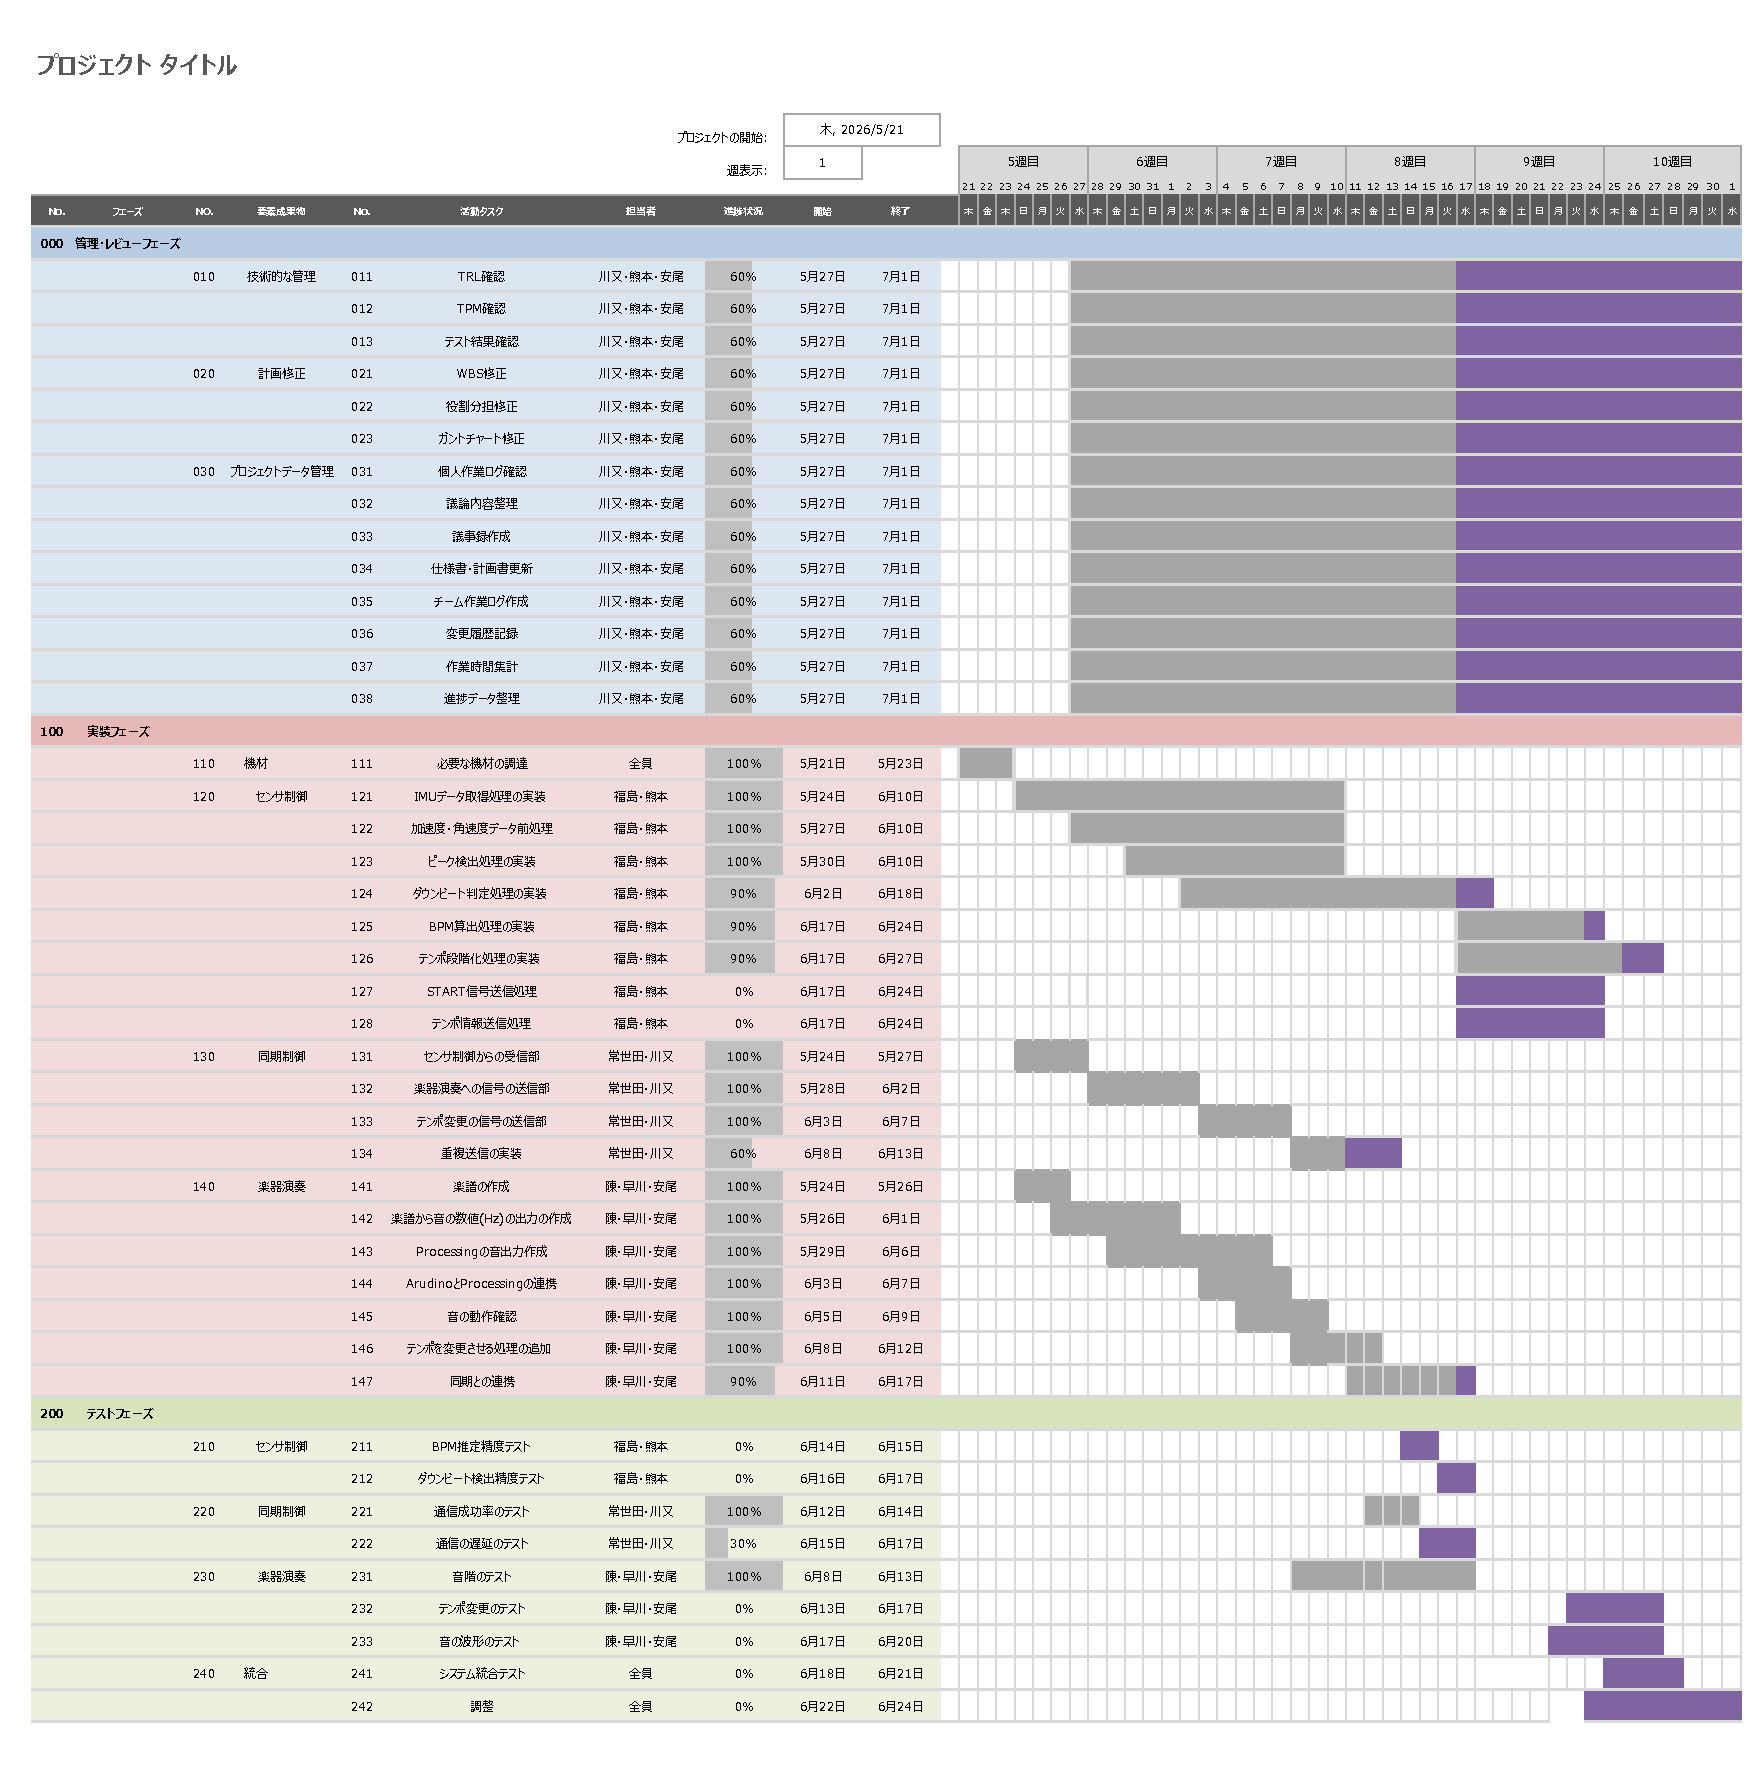
\includegraphics[width=0.8\textwidth]{gant8.pdf}
    \caption{ガントチャート}
\end{figure}

\section{日ごとの作業時間と作業内容}
今週実施した日ごとの具体的な作業時間および対応内容の詳細です．
\begin{table}[H]
    \centering
    \small
    \begin{tabular}{lll}
        \toprule
        日付 & 作業時間 & 作業内容 \\
        \midrule
        {}[6/20] & [2.0時間] & LEDマトリクス用カエルのドット絵(3コマ)の作成と検証用音源の準備． \\
        {}[6/22] & [2.0時間] & FrogMatrixの実装と，2つのinoへの共通組み込み・動作確認． \\
        {}[6/23] & [2.0時間] & librosaによる各音のピッチ検出と，目標音階との正解率の検証． \\
        \midrule
        \textbf{合計} & \textbf{[6.0時間]} & \\
        \bottomrule
    \end{tabular}
\end{table}

\section{課題管理}
\begin{table}[H]
    \centering
    \small
    \begin{tabular}{p{3cm}p{3cm}llp{3cm}ll}
        \toprule
        課題 & 発生原因 & 影響度 & 優先度 & 対策 & 期限 & 状態 \\
        \midrule
        実機での通信遅延・音ズレ & 無線通信の遅延が合奏の同期精度に影響する可能性 & 中 & 高 & 実機で遅延を測定し，許容範囲に収まるか確認する & [6/26] & 未着手 \\
        マトリクスと音の同期 & LEDアニメのコマ間隔(180ms)とテンポ変更時の見た目のずれ & 低 & 低 & テンポに連動した表示間隔の調整を検討する & [6/27] & 未着手 \\
        \bottomrule
    \end{tabular}
\end{table}
\vspace{0.5em}
\noindent ※影響度=プロジェクトへのインパクト，優先度=対応の緊急性

\section{AI 利用状況と検証(再現性重視)}
\subsection{利用内容}
\begin{itemize}
    \item 利用目的: \LaTeX による作業ログのテンプレート作成
    \item  入力(プロンプト要旨):
    \begin{itemize}
        \item 指定された作業ログのテンプレート項目の生成を依頼 ．
    \end{itemize}
    \item  出力概要:
    \begin{itemize}
        \item テンプレートの構成のコンパイル可能な作業ログの\LaTeX ソースコード ．
    \end{itemize}
\end{itemize}

\subsection{検証方法}
\begin{itemize}
    \item  検証手法: 生成された\LaTeX ソースコードの構造確認およびコンパイル検証
    \item  参照資料: 提供された作業ログテンプレートPDF
    \item  検証手順:
    \begin{enumerate}
        \item 生成されたコードのセクション構成が，テンプレート項目を漏れなく満たしているか目視で確認．
        \item \LaTeX 環境において実際にコンパイルを行い，エラーを吐かずに正しくPDFが生成されるかを確認．
    \end{enumerate}
\end{itemize}

\section{次回計画}
\begin{itemize}
    \item  目標: [実機での全体結合・音ズレ検証と，4台輪唱・LEDマトリクス・サーボを統合したデモの実施]
    \item  達成基準: [同期用Arduinoの無線コマンドで全楽器が再生・輪唱・テンポ変更でき，LEDマトリクスと音が同期し，音ズレが許容範囲に収まること]
    \item  期限: [7/1]
\end{itemize}

\section{その他}

\end{document}
